\section{Feature extraction}

In this section I will begin with a brief explanation of how the data is initially cleaned and then go on to explain how the features are extracted.\\

There are several ways of converting text into feature vectors suitable for input for the classification algorithms.
In this paper we compare the performance of encoding the sentences using character level n-grams and compare these results with feature vectors obtained using FastText.

\subsection{Bag of Words and one-hot encoding}
According to \cite{BagOfTricks} a simple and efficient base line for sentence classification is to represent sentences as a of words (BoW) and train a linear classifier.\footnote{The paper proposes logistic regression or an SVM} Here first a brief explanation of the BoW model. \\

Using words as features the first step of doing the BoW representation is to split each sentence into individual words. Continuing the example above the sentence would be split into.

\begin{verbatim}
['hesbjerg','er','dannet','ved',
'sammenlægning','af','de','gårde',
'store','hesbjerg','og','lille',
'hesbjerg','i']
\end{verbatim}

We proceed to make a dictionary over all the words in the the corpus (every word in the complete dataset) counting the frequency by which the each word appears. We can now sort the words by their frequency and in this way we can assign each word to a unique integer.

\begin{verbatim}
[2442,    3, 1513,   39,
 4819,   17,   30, 8684,
  189, 2442,    2,  617,
 2442,    1]
\end{verbatim}

Here we see that {\tt 'i', 'og'} and {\tt 'er' } are the most frequent words in the corpus.

Now for the one-hot encoding we construct a feature vector which has the dimension of the vocabulary and is zero everywhere except in the component corresponding to the integer which we have mapped the word onto as seen above. \\

When using individual word the vocabulary, and thus the dimension of the feature vector for each sentence, increases rapidly with the size of the dataset. In the example above using only 1000 sentences pr language the vocabulary consists of 26695 words and if use 50k sentences in each language the vocabulary grows to  368493!

\subsection{n-grams}

Apart from the large vocabulary, an obvious limitation of the bag of words model described above if that it does not take into account the relative position of each word.\\

A way to remedy this is to use character n-grams as features. An n-gram is constructed by regarding $n$ consecutive tokens (here either words or characters) as the features. An n-gram of size one is called a uni-gram and an n-gram of size 2 is called a bi-gram and so forth.\\

Continuing the example sentence above a bi-gram representation would look like

\begin{verbatim}
['he','es','sb','bj','je','er','rg','g ',
 ' e','er','r ',' d','da','an','nn','ne',
 'et','t ',' v','ve','ed','d ',' s','sa',
 'am','mm','me','en','nl','læ','æg','gn',
 'ni','in','ng','g ',' a',...]
\end{verbatim}

An advantage of using a character level representation instead of a word level is a drastic reduction in the vocabulary size. Since we only accept 40 characters a one-hot encoding using character level uni-grams would have at most 40 components while bi-grams would have a vocabulary of $40^2 = 1600$  and for trigrams the vocabulary would grow to  $40^3 = 64000$.\\

In this project we will compare the performance of a bag of words encoding using character level uni-grams and bi-grams with feature vectors obtained from using FastText.

\subsection{Using FastText}

The methods described above are quite simple and in this project i will also compare the above method with FastText which is a library for creating word embeddings developed by Facebook \cite{BagOfTricks}. \\

In the paper "Enriching Word Vectors with Subword Information" \cite{EnrichingWordVectors} the authors explain how FastText extracts feature vectors from raw text data. FastText makes word embedding using one of two model architectures: continuous bag of words (cbow) or the continuous skipgram model.\\

The skipgram and cbow models are first proposed in \cite{EfficientWordRepresentations} which is the paper introducing the word2vec model for word embeddings. FastText builds upon this work by proposing an extension to the skipgram model which takes into account subword information.\\

Both models use a neural network to learn word embedding from using a context windows consisting of the words surrounding the current target word. The CBOW architecture predicts the current word based on the context, and the skipgram predicts surrounding words given the current word.\cite{EfficientWordRepresentations} We see an illustration of this in Figure \ref{cbowskipgram}.

\begin{figure}[h!]
  \centering
  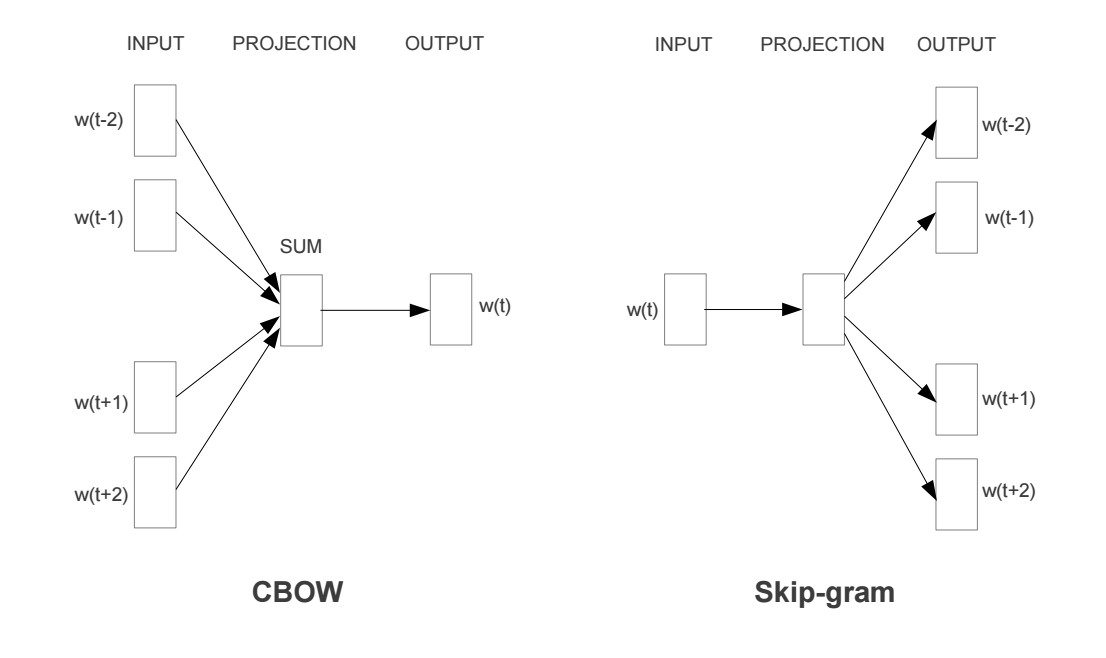
\includegraphics[width = 225pt]{figs/cbowskipgram}
  \caption{Diagram of the cbow and skipgram models.}
  \label{cbowskipgram}
\end{figure}



% % The order of context words does not influence prediction (bag-of-words assumption)
% Works by minimizing the-likelihood
%
% \begin{align}
% \sum_{t=1}^{T}\sum_{c}^{c \in C_t} \log p(w_c|w_t)
% \end{align}


% Skipgram vs continued bag of words.

% However, term frequencies are not necessarily the best representation for the text. Common words like "the", "a", "to" are almost always the terms with highest frequency in the text. Thus, having a high raw count does not necessarily mean that the corresponding word is more important. To address this problem, one of the most popular ways to "normalize" the term frequencies is to weight a term by the inverse of document frequency, or tf–idf. Additionally, for the specific purpose of classification, supervised alternatives have been developed to account for the class label of a document.[4] Lastly, binary (presence/absence or 1/0) weighting is used in place of frequencies for some problems (e.g., this option is implemented in the WEKA machine learning software system).
